%%%%%%%%%%%%%%%%%%%%%%%%%%%%%%%%%%%%%%%%%%%%%%%%%%%%%%%%%%%%%%%%%%%%%%%%%
%Objetivo: Realizar uma pesquisa com profissionais envolvidos em manutenção de
%		   software a fim de verificar a situação atual das funcionalidades
%		   oferecias pelas FGRM.
%Autor: Vagner Clementino<vagnercs@dcc.ufmg.br> e
%		Rodolfo Resende<rodolfo@dcc.ufmg.br>
%Data Criação: sex fev  3 19:57:56 BRST 2017
%Data Modificação: sáb abr 15 12:31:33 -03 2017
%Data Revisão: qui mai  4 20:50:59 -03 2017
%%%%%%%%%%%%%%%%%%%%%%%%%%%%%%%%%%%%%%%%%%%%%%%%%%%%%%%%%%%%%%%%%%%%%%%%%%
\chapter{Levantamento de Funcionalidades de FGRMs}\label{ch:pesquisa-profissionais}

\section{Introdução}\label{sec:pesquisa-profissionais-intro}

Neste capítulo apresentamos um levantamento por questionário com o objetivo de
coletar os aspectos mais importantes das funcionalidades oferecidas pelas FGRMs
do ponto de vista dos profissionais que trabalham com desenvolvimento e
manutenção de software. O planejamento e o desenho do estudo seguiram as
diretrizes propostas nos trabalhos de Wohlin~\cite{wohlin2012experimentation} e
Kasunic~\cite{kasunic2005designing}. Em especial, para selecionarmos a
população e a amostra de interesse utilizamos o arcabouço (framework) proposto
por De Mello e outros~\cite{de2015investigating, de2014towards}.

Para este levantamento foi definido que a população de interesse é a comunidade
envolvida com o processo de manutenção de software e que faça uso de FGRMs.
Pela abrangência e dificuldade de caracterização da população foi escolhida uma
amostra de conveniência. Neste sentido, utilizamos como amostra os
profissionais que estão envolvidos no projeto de código aberto
Python\footnote{\url{http://bugs.python.org/}}. Por outro lado, para tentarmos
coletar a opinião de profissionais com um conjunto de características que
esperamos ser mais abrangente, utilizamos os usuários da rede social de
desenvolvedores Stack Overflow\footnote{\url{http://stackoverflow.com}}. Neste
último caso, estamos interessados nos usuários da rede que tenham participado
de discussões sobre assuntos relacionados à manutenção de software.

A contribuição deste levantamento é que ele permitiu avaliar se os estudos
conduzidos na literatura que propõem melhorias que podem ser aplicadas para as
funcionalidades das FGRMs estão em consonância com as necessidades dos
profissionais. Neste sentido é possível analisar como está o distanciamento
entre o estado da arte e o da prática.

\section{Objetivo do Levantamento com Profissionais}\label{sec:objetivo_da_pesquisa_com_profissionais}

Em linhas gerais, o objetivo desta etapa da dissertação é analisar, através da
percepção e opinião dos profissionais envolvidos em Manutenção de Software, a
situação das funcionalidades atualmente oferecidas pelas FGRMs, bem como sobre
a adoção das metodologias propostas pelos agilistas no processo de manutenção
de software. Com intuito de atingir os objetivos propostos foram definidas as
seguintes questões de pesquisa:

% Colocando a finalidade do levantamento com base no método GQM (Goal, Question e
% Metric)\cite{gqm}, o propósito deste estudo \textit{é avaliar as
%     funcionalidades oferecidas pelas FGRMs e as melhorias propostas na
%     literatura, do ponto de vista dos profissionais envolvidos em Manutenção de
%     Software no contexto de projetos de software de código aberto e em empresas
%     publicas e privadas de informática.}

\begin{description}
	\item[Questão 01] Qual a opinião dos profissionais envolvidos em Manutenção
		de Software com relação as funcionalidades oferecidas pelas
		FGRM\@?
	\item[Questão 02] Na visão dos profissionais envolvidos em Manutenção de
        Software quais melhorias nas funcionalidades das FGRMs propostas na
        literatura teriam maior relevância em suas atividades?
	\item[Questão 03] As práticas propostas pelos agilistas estão sendo
        utilizadas no processo de Manutenção de Software?
    \item[Questão 04] Como as FGRMs podem ajudar as equipes de manutenção na
        adoção das práticas propostas pelos agilistas?
\end{description}

O desenho da pesquisa é detalhado na próxima seção onde discutimos a estrutura
do questionário bem como detalhamos o processo de seleção da amostra que foi
utilizado.

\section{Desenho e Método da Pesquisa com Profissionais}\label{sec:desenho_da_pesquisa_com_profissionais}

\subsection{Conceitos Básicos}

Estudos primários em Engenharia de Software (SE), como os levantamentos por
questionário, são muitas vezes conduzidos em amostras estabelecidas por
conveniência~\cite{sjoberg2005survey, dybaa2006systematic}. Um desafio na
determinação de amostras representativas, especialmente em Engenharia de
Software, é a identificação de fontes relevantes e disponíveis que permitam a
criação de amostragem~\cite{de2014towards}. Uma alternativa é a utilização de
fontes disponíveis na Internet, como rede sociais e projetos de código aberto,
que permitem aumentar o acesso à potenciais participantes~\cite{de2013would}.

O levantamento descrito neste capítulo consistiu de um estudo exploratório sem
uma hipótese prévia. Idealmente, ele deveria ser respondido por todos os
profissionais envolvidos com desenvolvimento e manutenção de software. Como não
é possível alcançar essa população, nos conformamos em utilizar uma
\textit{amostra de conveniência}. Neste tipo de amostragem a seleção de
indivíduos é realizada por conta de sua facilidade de acesso ou
proximidade~\cite{marshall1996sampling}. Este é um dos riscos à validade do
estudo e é discutido na Seção~\ref{subsubsec:fontes_amostragem}.

Para selecionarmos a amostra utilizado como base o estudo de Mello e
outros~\cite{de2014towards}. Nele os autores apresentam um arcabouço
(framework) conceitual para a determinação de fontes adequadas para amostragens
com foco em estudos na área de Engenharia de Software. Decidimos utilizar
alguns aspectos deste arcabouço para discutir a adequação da nossa amostra. O
modelo inclui termos estatísticos, tais como público-alvo, população,
amostragem e unidade de observação~\cite{thompson2012sampling}, e discute
conceitos como \textit{Fonte de Amostragem, Unidade de Pesquisa, Plano de
    Pesquisa e Estratégia de Amostragem}. No estudo os autores apresentam
alguns atributos, denominado Requisitos Essenciais~-~Essential Requeriments
(ER), que podem ser utilizadas para determinar que uma Fonte de Amostragem é
válida e que estão descritos a seguir.

% Segundo os autores, uma Fonte de Amostragem deveria ser organizada utilizando
% um sistema de banco de dados de modo a possibilitar a extração de subconjuntos
% que serão as amostras da população. Neste sentido, o estudo afirma que no caso
% de uma Fonte de Amostragem ser considerada pertinente para um contexto de
% pesquisa específico, pode-se concluir que as amostras extraídas desta fonte
% também podem ser consideradas válidas.

\begin{description}

    \item[ER1] Uma Fonte de Amostragem não deve representar intencionalmente um
               subconjunto segregado do público-alvo, ou seja, dado um
               público-alvo \textit{``X''}, não seria adequado pesquisar por
               unidades na fonte intencionalmente desenhada para compor um
               subconjunto específico de \textit{``X''}.

    \item[ER2] Uma Fonte de Amostragem não deve apresentar qualquer viés, como
               incluir na sua base de dados determinados subconjuntos do
               público-alvo.  Critérios desiguais para inclusão de Unidades de
               Pesquisa significam oportunidades desiguais para oportunidades
               de amostragem.

    \item[ER3] Todas as Unidades de Pesquisa\footnote{Uma Unidade de Pesquisa
               caracteriza como uma ou mais Unidade de Observação podem ser
               recuperadas de uma \textit{Fonte de Amostragem}.} das amostras e
               suas Unidades de Observação\footnote{Unidade de Observação é a
               entidade que é estudada em determinado experimento.}
               devem identificados de forma única.

    \item[ER4] Todas as amostragem de determinada Unidade de Pesquisa devem ser
               acessíveis. Se houver unidades de pesquisa ocultas,
               não é possível contextualizar a população.

\end{description}

\subsection{Método de Pesquisa}\label{subsec:pesq_metodologias}

No escopo deste levantamento, o público-alvo é o conjunto de profissionais que
trabalham com desenvolvimento e manutenção de software. Adicionalmente, seria
importante que o participante tivesse um mínimo de experiência de uso de alguma
FGRM\@. A caracterização e estratificação da população que temos interesse não
é simples. Neste sentido, é difícil dizer que um extrato com uma certa
experiência com FGRMs é mais relevante do que outro ou ainda questões como
processo de software ou linguagem de programação. Salvo melhor juízo, todos os
desenvolvedores de código aberto e código proprietário, que de alguma forma
tenham utilizado alguma FGRM, podem ser relevantes nesta investigação.

\subsubsection{Fontes de Amostragem}\label{subsubsec:fontes_amostragem}

Uma \textit{Fonte de Amostragem} corresponde a um banco de dados, não
necessariamente automatizado, em que um subconjunto válido da população pode
ser recuperado. Outra característica é permitir a extração aleatória de
amostras da população de interesse~\cite{de2014towards}. Utilizamos nesta
dissertação as duas Fontes de Amostragem exibidas na
Tabela~\ref{tab:fontes-amostragens}. Na primeira fonte, temos a expectativa de
encontrarmos indivíduos ligados ao desenvolvimento da linguagem Python que
correspondam ou representem profissionais do extrato de código aberto. A
segunda fonte, FA02, corresponde a indivíduos com interesse na rede social
Stack Overflow em que é possível que encontremos um perfil mais abrangente de
desenvolvedores e mantenedores de software\footnote{Não tentamos distinguir se
    o foco da atividade do usuário do Stack Overflow é desenvolvimento,
    manutenção ou outra categoria}.

\begin{table}[htpb]
\centering
\resizebox{.8\textwidth}{!}{%
\begin{tabular}{@{}lllc@{}}
\toprule
\textbf{Identificador} & \multicolumn{1}{c}{\textbf{Fonte de Amostragem}} &
\multicolumn{1}{c}{\textbf{URL}} \\ \midrule
FA01 & Python & https://bugs.python.org/ \\
FA02 & Stack Overflow & https://stackoverflow.com \\ \bottomrule
\end{tabular}%
}
\caption{Fontes de Amostragem utilizadas no estudo}\label{tab:fontes-amostragens}
\end{table}

A fonte FA01 foi utilizada por apresentar as seguintes características:
\textit{(i)} pelo menos 5 anos de existência; \textit{(ii)} comunidade bem
estabelecida, no sentido de um número relevante e participativo de
contribuidores e usuários; \textit{(iii)} permite acesso aos dados históricos
de suas RMs. Por outro lado, a fonte FA02 foi selecionada devido sua extensão:
envolve mais de 6 milhões de usuários e poderia nos fornecer o acesso a um
perfil abrangente de participantes.\footnote{Disponível em
    \url{http://stackexchange.com/sites}. Acessado em novembro de 2016.}.

O fato de utilizarmos amostras de conveniência pode resultar em limitações
devido a forma subjetiva que uma amostra pode ser escolhida. Uma amostra de
conveniência é útil especialmente quando a randomização não é possível, como no
caso de uma população muito grande ou de difícil
caracterização~\cite{boxill1997introduction}. No estudo conduzido por de Melo e
outros~\cite{de2014towards} são apresentados quatro elementos denominados
``Requisitos Essenciais'' que são utilizados para dar validade a uma fonte de
amostragem. Nossa avaliação é que as fontes utilizadas satisfazem os
requisitos. Os requisitos \textit{ER1} e \textit{ER2} são atendidos já que cada
membro vinculado a cada uma das FAs têm igual possibilidade de participação no
levantamento. O requisito \textit{ER3} foi atendido pela atribuição de um
identificador único para cada participante que foi coletado pelo processo de
extração. Considerando que as FAs consideram apenas usuários com o endereço
eletrônico público, o requisito \textit{ER4} é atendido já que os participantes
estão de alguma forma acessíveis.

\subsubsection{Construção das Fontes de Amostragem}\label{subsubsec:construcao_fonte_amostragem}

Cada Fonte de Amostragem (FA) utilizou uma estratégia distinta para a sua
construção. Para a FA01 utilizamos a lista de RMs disponível na Internet através
da FGRM do projeto\footnote{\url{http://bugs.python.com}}. No caso da FA02 a
fonte primária de informação são as discussões realizadas pelos seus usuários,
especialmente aquelas sobre a temática da Manutenção de Software. Em ambos os
casos foram coletados automaticamente os atributos:

\begin{itemize}
	\item Nome do Participante
	\item E-mail do Participante
	\item Data de Ação
	\item Tipo de Ação
\end{itemize}

O Tipo de Ação representa aquilo que o participante realizou na lista de
discussão ou na rede social. Exemplos de ação estão no relato ou solução de RM,
no caso da FA01 ou ainda responder a uma pergunta de determinada discussão, no
caso da FA02. O tipo e a data da Ação foram utilizados para avaliar se o
indivíduo estaria no conjunto final de potenciais participantes do estudo. Além
daqueles atributos, foram coletadas outras informações através do questionário
de pesquisa, como por exemplo a localização geográfica, o tempo de experiência,
o nome da função desempenhada, as principais atribuições, dentre outros.

No caso do Stack Overflow utilizamos para seleção dos participantes uma métrica
da própria rede social conhecida como
reputação\footnote{\url{http://stackoverflow.com/help/whats-reputation}}.
Trata-se de uma medida aproximada de quanto a comunidade avalia as
contribuições de um usuário. Neste trabalho ela foi utilizada como um dos
critérios de seleção do participante, que incluiu ainda a sua frequência de
participação em discussões sobre Manutenção de Software.

Para extrairmos os dados da rede social Stack Overflow utilizamos a interface de
busca avançada que a plataforma disponibiliza e que permite consultar e analisar
os dados de todos os sites da rede Stack
Exchange\footnote{\url{http://data.stackexchange.com/stackoverflow}}. A
interface possibilita a utilização da linguagem SQL para acesso aos dados. A
Figura~\ref{fig:stack-exchange} exibe uma tela da interface utilizada para
coleta dos dados.

\begin{figure}[htpb]
	\centering
	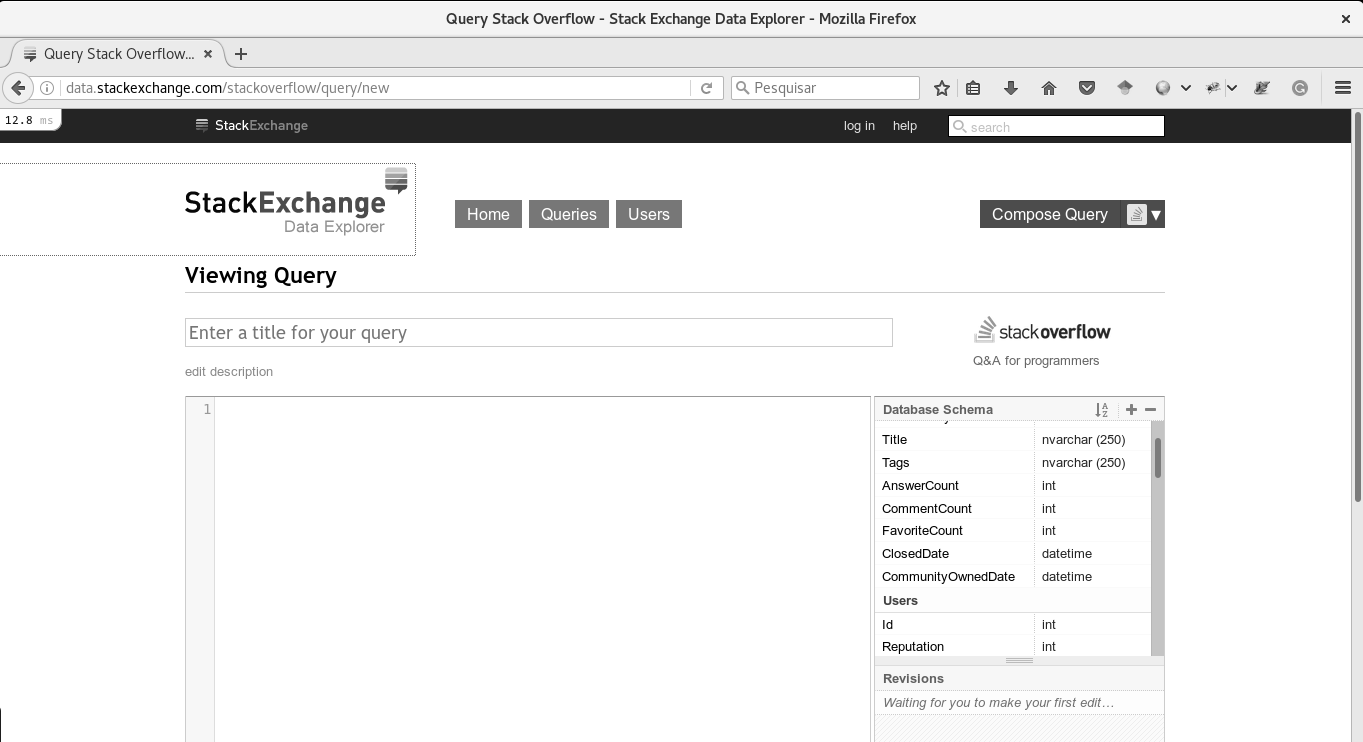
\includegraphics[width=0.7\linewidth]{./chapter-pesquisa-com-profissionais/img/stack-exchange.png}
	\caption{Ferramenta de coleta de dados da rede Stack Overflow}\label{fig:stack-exchange}
\end{figure}

Para a fonte FA01 foi desenvolvido um robô (web crawler) para coletar as
informações dos participantes. A partir de uma lista de RMs previamente
selecionada, a ferramenta coletou os dados dos possíveis participantes a partir
do histórico de modificações de cada RM\@. A
Figura~\ref{fig:historico-rm-python} apresenta o histórico de registros de uma
RM do projeto Python em que os dados dos participantes podem ser visualizados
nos quadros inseridos. Os dados coletados também foram armazenadas em um banco
de dados para posterior aplicação de critérios de inclusão e exclusão.

\begin{figure}[htpb]
	\centering
	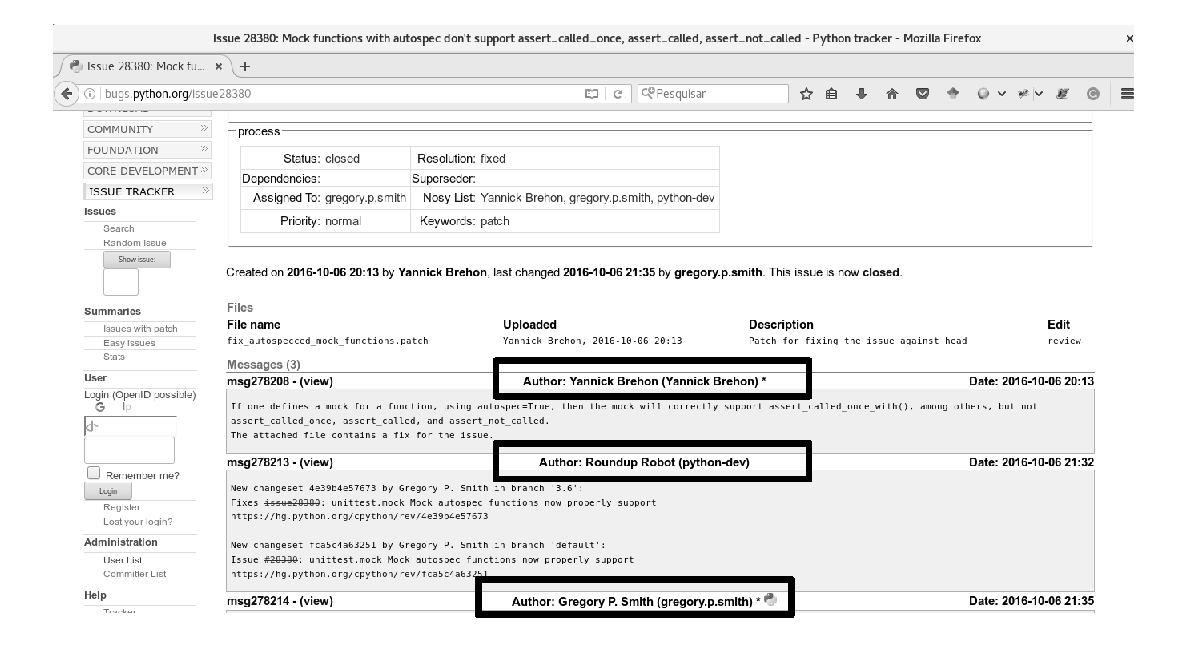
\includegraphics[width=0.7\linewidth]{./chapter-pesquisa-com-profissionais/img/historico-rm-python.pdf}
	\caption{Histórico de relatos de uma RM do projeto Python}\label{fig:historico-rm-python}
\end{figure}

\subsubsection{Seleção dos Participantes}\label{subsubsec:pesquisa_profissionais_plano_pesquisa}

Utilizamos estratégias distintas em cada fonte de amostragem para escolher os
potenciais participantes do levantamento. Para a fonte FA01 utilizamos os
registros históricos das RMs ocorridos nos últimos 05 anos. Além disso, foi
coletada a frequência que o participante teve contato com o projeto, como por
exemplo abertura, solução ou comentários em RMs. Um participante seria incluído
caso tivesse pelo menos uma interação no período avaliado.

No caso do Stack Overflow realizamos a busca de discussões com base nas
sentenças de busca exibidas na Figura~\ref{fig:setencas-grupos}. Um conjunto
similar de sentenças foi utilizado no mapeamento sistemático descrito no
Capítulo~\ref{ch:mapeamento-sistematico}. De modo a considerar as preferências
de privacidade dos indivíduos que iriam compor as Fontes de Amostragens, não
incluímos os participantes que proíbem a utilização dos seus dados,
especialmente do seu endereço eletrônico. Nesta mesma linha, não incluímos
pessoas que utilizam uma língua diferente do inglês, tendo em vista que apenas
existiam versões em inglês e português para o questionário utilizado no estudo.

\begin{figure}[htpb]
	\centering
	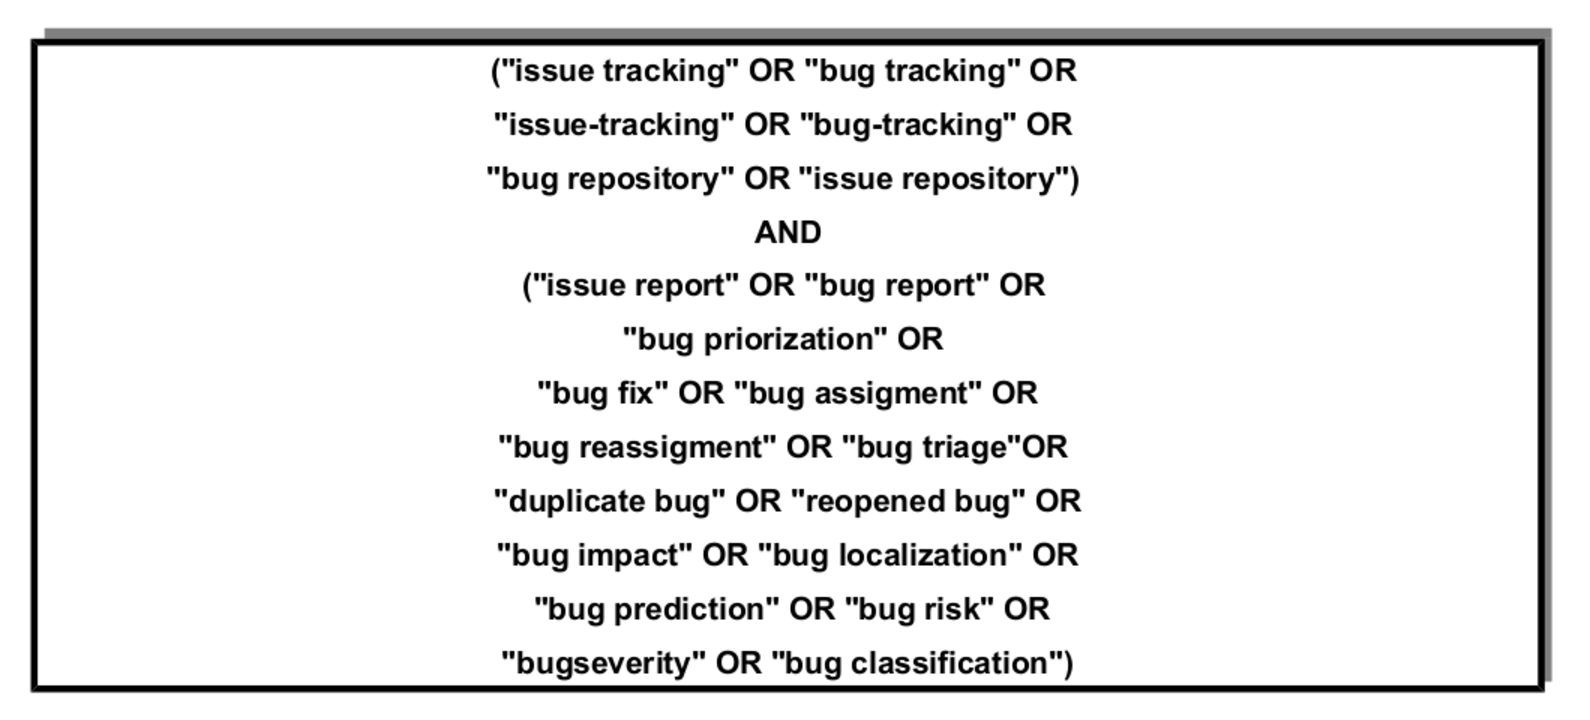
\includegraphics[width=0.7\linewidth]{./chapter-pesquisa-com-profissionais/img/setencas-grupos.pdf}
	\caption{Sentenças utilizadas para seleção das discussões no Stack Overflow}\label{fig:setencas-grupos}
\end{figure}

\subsubsection{Formulário}\label{subsubsec:questionario}

O formulário enviado aos participantes foi estruturado em três partes, cada uma
coletando um conjunto de informação. Na primeira estávamos interessados na
formação do participante. O segundo conjunto de perguntas tinha por objetivo
coletar a percepção dos participantes sobre as funcionalidades oferecidas pelas
FGRMs\@. Na terceira parte estão as perguntas sobre as melhorias e proposição de
novas funcionalidades para as FGRMs. Antes de aplicarmos o questionário foi
realizado um processo de avaliação constituído de quatro etapas:

\begin{enumerate}[(i)]
	\item Avaliação por Pesquisadores: Nesta etapa a primeira versão do
		formulário foi enviada para dois pesquisadores da área de manutenção de
		software.
	\item Avaliação por Profissionais: O formulário resultante da análise
		anterior foi encaminhado a dois profissionais que trabalham com
		manutenção de software.
	\item Piloto da Pesquisa: O formulário obtido da fase anterior foi utilizado
		em um piloto com dez profissionais envolvidos da manutenção de software
		de uma empresa pública de informática.
	\item Tradução do Formulário: Em cada uma das etapas anteriores o
		formulário foi aplicado em português, tendo em vista a falta de fluência
		em Inglês de alguns profissionais envolvidos no processo de avaliação,
		em especial na fase Piloto da Pesquisa. Neste sentido, a última etapa
		consistiu na tradução do formulário para a língua inglesa. Esta etapa
		foi conduzida com o suporte de um pesquisador experiente na área de
		Engenharia de Software.
\end{enumerate}

Após o processo de avaliação do questionário\footnote{A versão final do
    questionário pode ser encontrada em
    \url{https://archive.org/download/dissertacao-vagner-clementino-um-estudo/form-melhorias-funcionalidades.pdf}},
enviamos uma mensagem de correio eletrônico solicitando a colaboração com nosso
trabalho de mestrado. O gabarito (\textit{template}) da mensagem enviada pode
ser visualizado no Apêndice~\ref{ch:app-template-msg-pesquisa-profissionais}.
Foram enviadas um total de 452 mensagens de correio eletrônico no período de
02/01/2017 a 27/01/2017.

%\subsubsection{Envio da Mensagem}
%\label{subsubsub:envio_mensagem}

%A fim de viabilizar e mitigar os riscos operacionais do envio manual de
%mensagens ao participantes foi desenvolvido um processo automatizado de remessa
%de mensagens aos participantes. O processo seguiu uma política que consiste em
%enviar uma mensagem ao participante com base em um modelo. Após um um prazo de
%dois dias uma nova mensagem era enviada. Foi construída uma lista para incluir o
%endereço eletrônico daqueles que não gostariam de receber lembretes ou de
%participar da pesquisa de modo a respeitar a privacidade do participante. As
%mensagens foram preenchidas (uma a uma) e enviadas por meio de correio
%eletrônico com base no seguinte modelo:

%\fbox{\begin{minipage}{\textwidth}
%Dear \{\{ nome do participante\}\}\!

%I’m Vagner Clementino (\url{homepages.dcc.ufmg.br/~vagnercs}), Master Student at
%Federal University of Minas Gerais, Brazil. I’m conducting a research,
%supervised by Prof\. Rodolfo Resende \@-\@ \url{homepages.dcc.ufmg.br/~rodolfo}
%concerned with improvements in Issue Tracking System. As part of them, we
%planned and executed a survey aiming at to reaching a large-scale population of
%researchers/practitioners interested on the improve the features of the Issue
%Tracking Systems. Based on your area of interest, we kindly invite you to take
%part in the following survey:

%\{\{url do formulario\}\}

%You were chosen because your relevant participation/contribution in \{\{nome da
%fonte de amostragem\}\}\@-\@ \{\{url da fonte de amostragem\}\}. Your opinion is
%essential to strength our findings. Please, help us accordingly to your
%possibilities by answering this survey until \{\{data limite\}\}. As soon as we
%conclude the data analysis, we will share the results with all participants and
%the software engineering community. If you have already fulfilled this
%questionnaire, please ignore this email.

%Thanks in advance,\\
%Vagner Clementino\\

%\end{minipage}}

\section{Resultados}\label{sec:analise_dados}

Nesta seção apresentamos os resultados obtidos na aplicação do questionário.
Após o envio das mensagens obtivemos 85 participações. É importante salientar
que nenhuma das questões do formulário era de preenchimento obrigatório, desta
forma, alguns dos resultados não necessariamente vai apresentar o total de
respostas recebidas. Começamos com a análise do perfil dos respondentes. Em
seguida, avaliamos o nível de satisfação com as ferramentas que utilizam.
Posteriormente verificamos o grau de adoção das metodologias propostas pelos
agilistas no processo de desenvolvimento e manutenção de software.

\subsection{Perfil dos Participantes}\label{sub:pesquisa_prof_perfil_dos_participantes}

O tipo de atividade realizada pelos participantes pode ser visualizado na
Tabela~\ref{tab:grafico_melhorias_fgrm_funcao_particantes}. A função com mais
frequência de participações é a de desenvolvedor, o que corresponde a cerca de
um terço dos participantes. Todavia, grande parte dos respondentes pode estar
envolvida com tarefas de desenvolvimento e manutenção de software, tanto que
mais de 80\% da amostra é formada por desenvolvedores, engenheiros de software,
gerentes e arquitetos.

\begin{table}[htpb]
\centering
\resizebox{.4\textwidth}{!}{%
\begin{tabular}{@{}lc@{}}
\toprule
\textbf{Função Desempenhada} & \textbf{Total} \\ \midrule
Desenvolvedor & 23 \\
Engenheiro de Software & 17 \\
Gerente & 12 \\
Arquiteto de Software & 5 \\
Pesquisador & 5 \\
Consultor & 4 \\
Estudante & 3 \\
Analista de Qualidade & 1 \\
Designer & 1 \\ \bottomrule
\end{tabular}%
}
\caption{Função desempenhada pelos participantes}\label{tab:grafico_melhorias_fgrm_funcao_particantes}
\end{table}

A distribuição geográfica dos participantes demostra uma proeminência de
pessoas da Ásia (32\%), Europa (27\%) e em seguida das América do Norte (17\%)
e América do Sul (12\%). A
Tabela~\ref{tab:melhorias_fgrm_localizacao_geografica} exibe o total de
participações pela localização geográfica. Esta distribuição pode atenuar
possíveis enviesamentos que por ventura algum nicho geográfico possa
apresentar. Todavia, não está no escopo deste estudo discutir como que as
diferenças de localização do participante podem influenciar nos resultados. Os
respondentes trabalham em sua maioria em empresas privadas de software (74\%).
Existem também aqueles que participam de projetos de código aberto (6\%) e
empresa pública de software (4\%). O restante do grupo que respondeu esta
questão é composto por contribuidores de projetos de software livre e
estudantes. É importante considerar que grande parte dos respondentes pertencem
à empresas privadas, em que os processos e ferramentas não podem ser
modificados pelo desenvolvedor. Esta característica pode afetar os resultados,
especialmente quando avaliarmos o nível de satisfação das funcionalidades das
FGRMs.

\begin{table}[htpb]
\centering
\resizebox{.4\textwidth}{!}{%
\begin{tabular}{@{}lc@{}}
\toprule
\textbf{Localização} & \textbf{Participações} \\ \midrule
Asia                 & 28                     \\
Europa               & 23                     \\
América do Norte     & 15                     \\
América do Sul       & 11                     \\
Africa               & 4                      \\
América Central      & 2                      \\
Oceania              & 2                      \\ \bottomrule
\end{tabular}%
}
\caption{Localização Geográfica dos Participantes}\label{tab:melhorias_fgrm_localizacao_geografica}
\end{table}

A equipe que o participante faz parte possui em geral mais de dez componentes
(31\%). Em segundo lugar, temos equipes de médio porte, entre seis e dez
membros (28\%). A Tabela~\ref{tab:melhorias_fgrm_tamanho_equipe} apresenta a
frequência de respostas para o tamanho da equipe. Os participantes possuem com
maior frequência entre três e dez anos de experiência. Existem ainda 09
participantes que possuem mais de dez anos trabalhando com desenvolvimento ou
manutenção de software. Em síntese, temos um grupo com significativa
experiência o que pode agregar valor aos resultados finais.

\begin{table}[htpb]
\centering
\resizebox{.6\textwidth}{!}{%
\begin{tabular}{@{}lc@{}}
\toprule
\textbf{Tamanho da Equipe} & \multicolumn{1}{l}{\textbf{Número de Respostas}} \\ \midrule
Mais do que 10 & 23 \\
Entre 6 e 10 & 21 \\
Entre 2 e 5 & 1 \\
1 (eu mesmo) & 13 \\ \bottomrule
\end{tabular}%
}
\caption{Tamanho da equipe dos participantes}\label{tab:melhorias_fgrm_tamanho_equipe}
\end{table}

% Em resumo as respostas tipicamente vieram de desenvolvedores, localizados na
% Ásia e Europa, com um tempo de experiência entre três e dez anos, trabalhando em
% uma equipe com aproximadamente dez membros. A partir deste perfil entendemos que
% foi possível alcançar uma amostra com um perfil adequado para responder as
% questões propostas.

\subsection{Nível de Satisfação com as FGRM}\label{sub:nivel_de_satisfação_com_as_fgrm}

A avaliação da ferramenta utilizada pelo participante é importante tendo em
vista que as opiniões dadas podem estar relacionadas com a versão utilizada,
podendo os resultados se mostrarem diferentes se a pesquisa fosse realizada com
outras versões dos sistema. A maior frequência ocorre para a ferramenta
\textit{Jira (28\%)}. Na segunda posição visualizamos o \textit{Github (17\%)}
que é um serviço de web para armazenamento de projetos que usam o controle de
versionamento \textit{Git} e que possui um módulo que oferece funções
existentes nas FGRMs. Uma outra ferramenta bem posicionada foi o \textit{Trello
    (10\%)}, que é um software de planejamento no estilo \textit{Kanban} e que
segundo os nossos resultados está sendo utilizado para gestão das RMs. Um
conjunto de dezenove ferramentas, correspondendo a um total de 32\% das
respostas, foram escolhidas uma única vez, dando um indício da extensão das
FGRMs disponíveis.

% \begin{figure}[htpb]
% 	\centering
% 	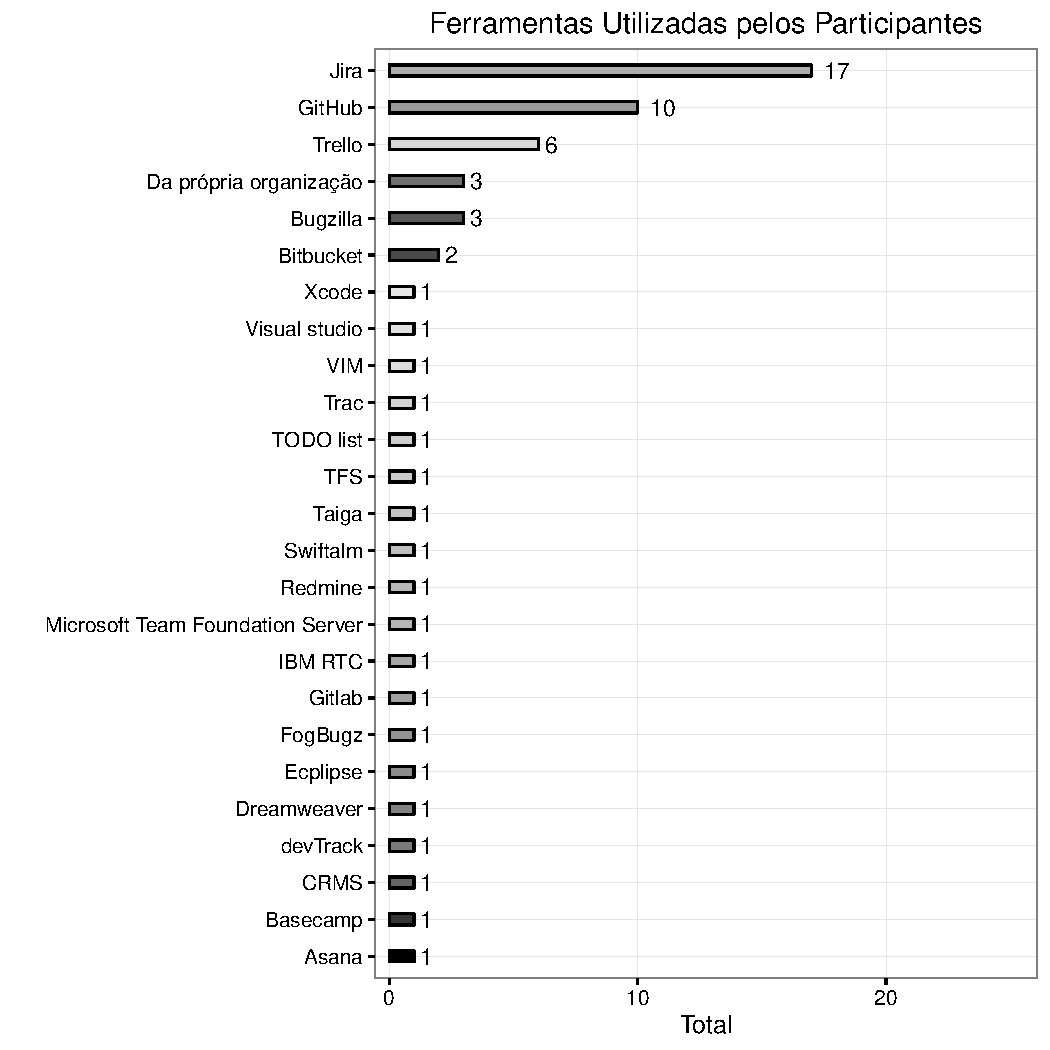
\includegraphics[width=0.5\linewidth]{./chapter-pesquisa-com-profissionais/img/grafico_melhorias_fgrm_ferramentas_utilizadas.pdf}
% 	\caption{Ferramentas utilizadas pelos participantes}
% \label{fig:grafico_melhorias_fgrm_ferramentas_utilizadas}
% \end{figure}

Verificamos o nível de satisfação dos participantes com as funcionalidades
oferecidas pelas FGRMs que ele utiliza. Em grande parte os respondentes estão
satisfeitos com as funcionalidades. A resposta com maior frequência foi
\textit{Nem satisfeito ou insatisfeito}, com cerca de 32 (44\%) respostas. Na
segunda posição, 21 profissionais (29\%) responderam que estão
\textit{Satisfeitos}. A opção \textit{Muito satisfeito} foi escolhida por 11
(15\%) dos profissionais. As alternativas que podem refletir uma insatisfação
sobre as funcionalidades (\textit{Desapontado ou Muito Desapontado}) foram
escolhidas por 8 (11\%) participantes. O item \textit{desapontado} teve 6
respostas e a opção \textit{Muito Desapontado} foi escolhida por 2
participantes. Se desconsiderarmos aqueles que selecionaram \textit{Nem
    satisfeito ou insatisfeito}, é possível verificar que a maior parte dos
respondentes (44\%) estão satisfeitos com as funcionalidades da FGRM que
utiliza. Em contrapartida, os participantes insatisfeitos representam 11\% da
amostra. O número de respostas não nos permite generalizar o resultado,
entretanto, ele não segue o que a literatura sobre melhorias em funcionalidades
das FGRMs em que se discute um possível descontentamento dos usuários deste
tipo de software. Uma possível explicação seria o desconhecimento dos
profissionais de funcionalidades que estão sendo propostas na literatura que
podem melhorar as suas atividades.

No mesmo questionário verificamos se o respondente recomendaria a ferramenta
que utiliza para outro projeto. A probabilidade de recomendação é exibida na
Tabela~\ref{tab:grafico_melhorias_fgrm_probabilidade_recomentacao}. De maneira
similar ao nível de satisfação grande parte dos participantes tendem a
recomendar a FGRM\@. Com base neste resultado, podemos deduzir que os
profissionais estão realmente satisfeitos com as funcionalidades da ferramenta
que utilizam ao ponto de recomendá-la.

\begin{table}[htpb]
\centering
\resizebox{.5\textwidth}{!}{%
\begin{tabular}{@{}lc@{}}
\toprule
\textbf{Recomendação da Ferramenta Utilizada} & \textbf{Total} \\ \midrule
Com certeza & 22 \\
Provável & 32 \\
Pouco Provável & 9 \\
Muito Improvável & 3 \\
Não Recomendaria & 5 \\ \bottomrule
\end{tabular}%
}
\caption{Probabilidade de Recomendação da Ferramenta Utilizada}\label{tab:grafico_melhorias_fgrm_probabilidade_recomentacao}
\end{table}

\subsection{Avaliação das Funcionalidades Existentes}\label{sub:avaliação_das_funcionalidades_existentes}

Nesta seção apresentamos a opinião dos profissionais sobre as funcionalidades
oferecidas atualmente pelas FGRMs\@. O conjunto de funcionalidades apresentado
ao participante é o resultado do estudo descrito na
Seção~\ref{sec:caracterizacao_ferramentas}. No questionário apresentamos ao
participante uma lista de funcionalidades e pedimos que para cada uma fosse
escolhida um item de uma escala de importância (\textit{Nada Importante, Pouco
    Importante, Importante, Levemente Importante, Muito Importante}). Com base
nas respostas, as seguinte funcionalidades foram consideradas como as mais
importantes: \textit{Suporte ao Unicode, Múltiplos Projetos, Integração com
    Sistemas de Controle de Versão (VCS Integration)}.

% \begin{table}[htpb]
% \centering
% \resizebox{\textwidth}{!}{%
% \begin{tabular}{@{}lccccc@{}}
% \toprule
% \multicolumn{1}{|c|}{\multirow{2}{*}{\textbf{Funcionalidade}}} &
% \multicolumn{5}{c|}{\textbf{Classificação}} \\ \cmidrule(l){2-6}
% \multicolumn{1}{|c|}{} &
% \multicolumn{1}{c|}{\textbf{\begin{tabular}[c]{@{}c@{}}Nada \\
%             Importante\end{tabular}}} &
% \multicolumn{1}{c|}{\textbf{\begin{tabular}[c]{@{}c@{}}Pouco\\
%             Importante\end{tabular}}} & \multicolumn{1}{c|}{\textbf{Importante}}
% & \multicolumn{1}{c|}{\textbf{\begin{tabular}[c]{@{}c@{}}Levemente\\
%             Importante\end{tabular}}} &
% \textbf{\begin{tabular}[c]{@{}c@{}}Muito\\ Importante\end{tabular}} \\ \midrule
% Integração com a documentação de software & 11 & 12 & 15 & 12 & 14 \\
% Integração com plano de teste & 11 & 13 & 13 & 13 & 9 \\
% Fluxo de trabalho customizável & 9 & 14 & 21 & 14 & 15 \\
% Suporte à Unicode & 9 & 9 & 21 & 16 & 24 \\
% Campos customizáveis & 5 & 17 & 25 & 22 & 8 \\
% Suporte ao Acordo de Nível de Serviço (SLA) & 14 & 22 & 15 & 13 & 10 \\
% Extensões (plugins) / APIs para integração com outros produtos & 8 & 14 & 21 & 19 & 16 \\
% Suporte à múltiplos projetos & 3 & 8 & 17 & 21 & 28 \\
% Busca textual & 1 & 5 & 17 & 15 & 40 \\
% Busca por arquivos & 4 & 15 & 18 & 17 & 24 \\
% Integração com Sistemas de Controle de Versão & 7 & 16 & 16 & 13 & 21 \\
% Múltiplas interfaces de notificações (E-mail, RSS, XMPP, etc) & 7 & 11 & 23 & 16 & 19 \\
% Suporte à Revisão de Código & 2 & 2 & 0 & 0 & 5 \\
% Facilidade de Uso & 0 & 2 & 2 & 0 & 1 \\
% Integração com bancos de dados & 4 & 6 & 4 & 1 & 2 \\ \bottomrule
% \end{tabular}%
% }
% \caption{Avaliação da importância das funcionalidades pelos profissionais}\label{tab:avaliacao_funcionalidades}
% \end{table}

Por outro lado, apresentamos aos profissionais funcionalidades que poderiam ser
integradas à FGRM que ele utiliza. As funcionalidades foram baseados na
literatura da área, tomando com base o Mapeamento Sistemático descrito no
Capítulo~\ref{ch:mapeamento-sistematico}. A
Figura~\ref{fig:grafico_melhorias_fgrm_funcionalidades_falantes} apresenta as
funcionalidades que os participantes sentem falta. As funcionalidades foram
apresentadas aos profissionais através de uma lista e foi permitido que eles
escolhessem mais de uma opção. O resultado nos mostrou que funções tais como
\textit{Identificação Automática de RMs Duplicadas, Atribuição Automática de RM
    e Análise de Impacto} foram as mais bem avaliadas.

% \begin{table}[htpb]
% \centering
% \resizebox{\textwidth}{!}{%
% \begin{tabular}{@{}lc@{}}
% \toprule
% \multicolumn{1}{c}{\textbf{Novas Funcionalidades}} & \textbf{Ranking} \\ \midrule
% A ferramenta deve permitir buscar por RM's duplicadas incluindo, &
% \multirow{2}{*}{1} \\ por exemplo, a possibilidade de busca por expressões
% regulares. &  \\ \midrule A ferramenta deve  coletar as informações que os
% desenvolvedores & \multirow{2}{*}{2} \\ necessitam para solucionar a RM\@. &  \\
% \midrule A ferramenta deve introduzir o conceito de reputação nos perfis &
% \multirow{2}{*}{3} \\ dos usuários. As RMs relatadas por usuários com boa
% reputação teriam prioridade. &  \\ \midrule A ferramenta deve guiar os usuários
% no processo de relatar RMs, por exemplo, & \multirow{2}{*}{4} \\ ajudando aos
% reportadores menos experientes na coleta de informações relevantes. &  \\
% \midrule A ferramenta deve permitir a tradução de RMs  descritas em outro
% idioma. & 5 \\ \midrule As FGRMs deveriam ``premiar'' os reportadores quando
% eles realizarem & \multirow{2}{*}{6} \\ um relato de qualidade. &  \\ \bottomrule
% \end{tabular}%
% }
% \caption{Novas Funcionalidades para as FGRMs}
% \label{tab:novas_funcionalidas_para_fgrms}
% \end{table}


\begin{figure}[htpb]
	\centering
	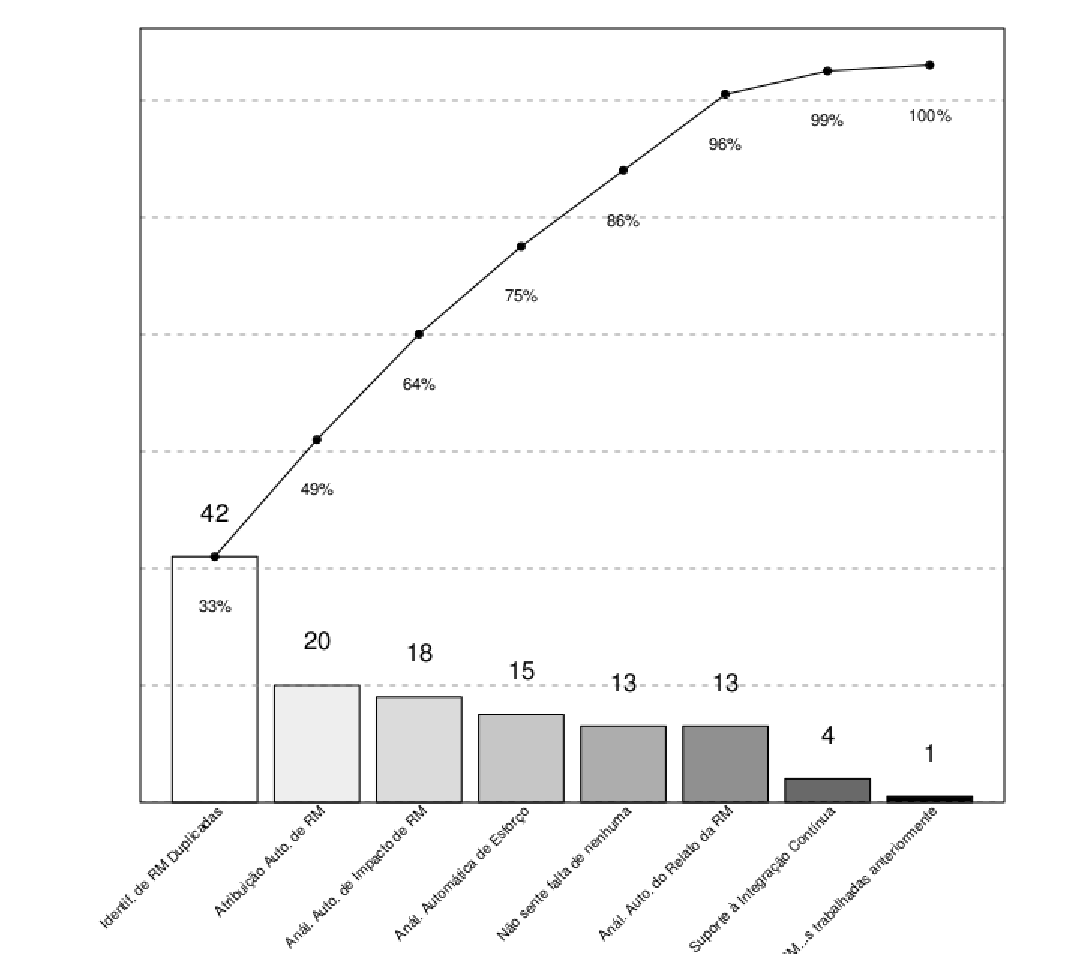
\includegraphics[width=0.9\linewidth]{./chapter-pesquisa-com-profissionais/img/grafico_melhorias_fgrm_funcionalidades_faltantes.eps}
	\caption{Funcionalidades que o participantes sentem falta.}\label{fig:grafico_melhorias_fgrm_funcionalidades_falantes}
\end{figure}

\subsection{Práticas Ágeis na Manutenção de Software}\label{sub:práticas_ágeis_na_manutenção_de_software}

Nesta etapa do levantamento com profissionais, estamos interessados em analisar
como as práticas propostas pelos agilistas estão sendo utilizadas no
desenvolvimento e em especial na manutenção de software. Após a apresentação de
um cardápio de opções, obtidas de um livro sobre metodologias
ágeis~\cite{meyer2014agile}, os participantes selecionaram como as práticas
mais adotadas: \textit{Integração Contínua} (17\%), \textit{Padrões de
    Programação} (16\%), \textit{Refatoração} (15\%), \textit{Reunião Diária
    (daily)} (13\%) e \textit{Propriedade compartilhada de código} (10\%).

A fim de avaliar como as FGRMs podem ajudar as equipes de manutenção de
software na adoção das práticas propostas agilistas, apresentamos aos
participantes do levantamento uma lista de possíveis funcionalidades com este
viés. Foi solicitado a eles escolhessem a ordem em que estas melhorias seriam
implementadas na ferramenta que utiliza, sendo 1 a maior prioridade e 7 a
menor. Segundo o nosso entendimento as funções que tivessem uma maior
prioridade para serem implementadas poderiam ser consideradas mais relevantes
para os profissionais. A Tabela~\ref{tab:melhorias_fgrm_suporte_particas_ageis}
apresenta a opinião dos profissionais sobre as funcionalidades mais relevantes.
Segundo eles, a priorização automática de RMs urgentes e não esperadas, ajuda o
desenvolvedor nas reuniões diárias e o suporte a tarefas compartilhadas foram
as respostas mais frequentes.

\begin{table}[htpb]
\centering
\resizebox{\textwidth}{!}{%
\begin{tabular}{@{}lc@{}}
\toprule
\textbf{Melhorias Propostas} & \multicolumn{1}{l}{\textbf{Classificação}} \\
\midrule Priorização automatizada de RMs  urgentes e inesperadas & 1 \\ Sugestão
automatizada das  RMs que farão parte da iteração. & 2 \\ Suporte aos
desenvolvedores na  preparação para reunião diária & 3 \\ Suporte à
divisão de tarefas de forma compartilhada & 4 \\ Facilitar a propriedade
compartilhada de código & 5 \\ \bottomrule \end{tabular}%
}
\caption{Classificação das funcionalidades que possam dar suporte ao uso das
metodologias dos agilistas.}\label{tab:melhorias_fgrm_suporte_particas_ageis}
\end{table}

\section{Discussão}

\paragraph{Nível de Satisfação com a Ferramenta Utilizada:}\label{par:pesq_profissionais_nivel_de_satisfação}

Em geral, o nível de satisfação com as funcionalidades oferecidas pelas FGRMs é
alto. Esta medida foi observada na análise do nível da satisfação dos
participantes em que verificamos que cerca de 44\% estão de alguma forma
satisfeito com a ferramenta que utilizam. Em contrapartida, os participantes
que mostraram algum tipo de insatisfação representaram 11\% da amostra. Este
mesmo sentimento pode ser observado pela alta probabilidade de recomendação da
FGRM utilizada para um novo projeto. Naquela medida verificamos que o mesmo
percentual de participantes pretende recomendar o software que utiliza.

\paragraph{Funcionalidades Faltantes:}\label{par:pesq_profissionais_funcionalidades_faltantes}

Apesar dos profissionais estarem satisfeitos com as funcionalidades ofertadas
pela FGRM que utiliza, quando lhe foi apresentado um conjunto de novas funções
grande parte deles aprova a inclusão de algumas delas. Por exemplo, cerca de um
terço dos participantes disseram sentir falta de um processo de identificação
automatizada de RMs duplicadas. Este resultado também foi encontrado no
trabalho de Zimmermann e outros~\cite{zimmermann2010makes} que ao conduzir um
levantamento com questionário em que o problema da duplicação de RMs foi
descrito como um dos problemas que pode ocasionar em atrasos na solução das
RMs.

Um ponto interessante é que as funcionalidades que os participantes mais
sentiram falta, também representam a maior quantidade de estudos na literatura.
Posto de outra forma, a automatização da detecção de RMs duplicadas e
atribuição de RMs são as soluções mais demandadas e representam o maior número
de trabalhos na literatura. Este resultado pode sugerir a necessidade de uma
maior divulgação do que está sendo proposto na literatura tendo em vista que os
profissionais se mostraram interessados nestes tipos de funcionalidades.

\paragraph{Suporte às Práticas dos Agilistas:}\label{par:pesq_profissionais_suporte_pratica_agilistas}

Apesar de ser pouco discutido na literatura, as FGRMs podem oferecer suporte às
praticas propostas pelos agilistas. Os participantes se mostraram interessados
em funções tais como a priorização automática de RMs urgentes e não esperadas,
ajuda na reunião diária e o suporte a tarefas compartilhadas. Com a crescente
adoção das práticas dos agilistas por equipes de desenvolvimento e manutenção de
software seria importante que este tipo de ferramenta incorporasse em suas
funcionalidades tal tendência. Conforme discutido na
Seção~\ref{sec:caracterizacao_ferramentas} as FGRMs, em sua maioria, não
apresentam funcionalidades que suportem as práticas propostas pelos agilistas.

\section{Ameaças à Validade}\label{sec:pesquisa_profissionais_ameacas_validade}

Uma ameaça à validade deste trabalho está no número de respondentes da pesquisa.
Apesar do esforço de seleção de uma amostra representativa da população o número
de participantes limita a extrapolação do resultados. O fato de ter sido
utilizada uma amostragem de conveniência implica que as generalizações são
limitadas já que a amostra pode não representar a população. Por outra lado,
utilizamos o arcabouço proposto por de Mello~\cite{de2014towards} visando
minimizar a introdução de enviesamento na amostra.

Ainda avaliando o processo de escolha das amostras utilizadas, não temos
garantias que as regras para seleção de participantes resultaram em um conjunto
bem representativo da população. Vale ressaltar que todas as opiniões coletadas
devem levar em conta a ferramenta que o profissional utilizava quando da
aplicação do questionário. Caso este mesmo estudo fosse realizado com outras
versões do mesmo sistema os resultados poderiam ser diferentes. Neste sentido,
a generalização dos resultados deve passar por esta característica do estudo.

\section{Resumo do Capítulo}\label{sec:resumo_do_capitulo}

Neste capítulo realizamos um levantamento mediante questionário com o objetivo
de entender e analisar a opinião de profissionais de desenvolvimento e
manutenção de software sobre as funcionalidades oferecidas pelas FGRMs. O
questionário foi preenchido por 85 participantes o que nos permitiu observar que
existia um bom nível de aceitação das funcionalidades no momento da realização
do estudo. Em contrapartida, quando apresentadas melhorias das funcionalidades
da ferramenta, muito dos desenvolvedores se mostraram interessados. As propostas
de melhorias foram baseadas nos resultados obtidos do Mapeamento Sistemático
descrito no Capítulo~\ref{ch:mapeamento-sistematico}. Este fato pode ilustrar a
necessidade de que os estudos propostos na literatura se integrem nas
ferramentas, através de protótipos, por exemplo, de modo a atender as
necessidades dos profissionais.
